\documentclass[margin=1pt]{standalone}

\usepackage{tikz}

\usetikzlibrary{
  calc, math,
}

\begin{document}
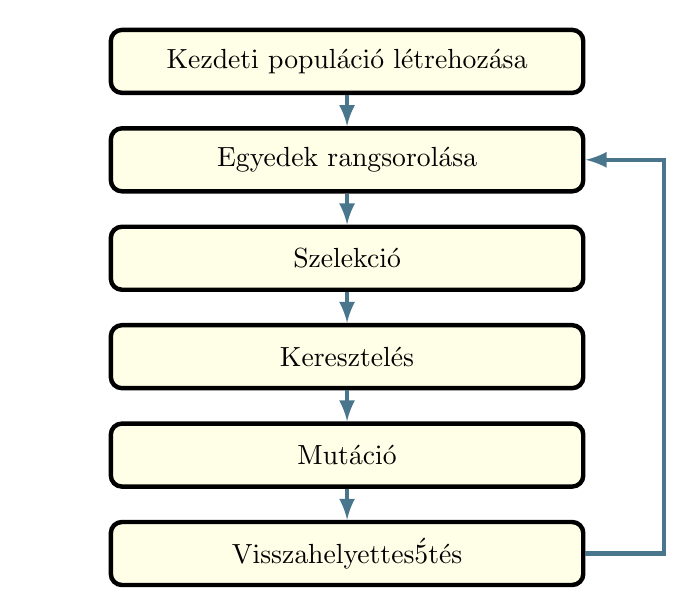
\begin{tikzpicture}[
    ultra thick,
    box/.style={
        rectangle, rounded corners,
        minimum height=.8cm, minimum width=6cm,
        draw=black, fill=yellow!10,
      },
    arr/.style={
        cyan!50!black, ultra thick,
      }
  ]
  \def\z{0}
  \foreach \i/\n in {
      0/Kezdeti populáció létrehozása,
      1/Egyedek rangsorolása,
      2/Szelekció,
      3/Keresztelés,
      4/Mutáció,
      5/Visszahelyettesítés
    }{
      \node[box] (\i) at (0,-1.25*\i) {\n};
      \ifx\i\z
      \else
        \draw[arr, evaluate={\o=int(\i-1);}, -latex] (\o) -- (\i);
      \fi
    }

  \draw[arr, -latex] (5.0) -- ++(1,0) |- (1);
  \draw[transparent] (5.180) -- ++(-1,0) |- (1);
\end{tikzpicture}
\end{document}
